\chapter{APPROCHE PROPOSÉE, MÉTHODOLOGIE ET ÉCHÉANCIER}

L'objectif consiste à définir et valider une méthode d'encodage textuel capable de représenter de façon fidèle et précise les dimensions visuelles, auditives et narratives d'une vidéo. Le tout, en restant assez concis pour permettre que le traitement soit fait par un LLM le moins énergivore possible et en utilisant le moins de jetons possible. Une des hypothèses sur laquelle repose cette partie est qu'avec une représentation suffisamment détaillée et avec un choix judicieux des composantes détaillées, le problème d'analyse vidéo pourrait être simplifié, permettant à un modèle moins puissant de l'analyser correctement. En bref, il s’agit d’encoder à l’avance les données jugées pertinentes, pour réduire la charge d’inférence du LLM.

La question de examine s'il est possible de générer une description textuelle suffisamment exhaustive d'une vidéo pour permettre à un grand modèle de langage (LLM) purement textuel d'identifier automatiquement les moments saillants d'une vidéo, dans le but de minimiser les ressources nécessaires pour l'analyse et pour l'utiliser dans des systèmes embarqués ou des situations de ressources limitées.

La première étape consiste à élaborer une représentation textuelle structurée du contenu vidéo, la deuxième étape évalue la capacité d'un LLM à identifier les segments clés à partir de cette représentation, la troisième étape compare les résultats obtenus avec des références existantes, et enfin, la quatrième étape met en place un processus itératif d'optimisation pour améliorer la précision et l'efficacité de l'approche.

\section{Élaboration d'une représentation textuelle structurée}

La représentation textuelle inclurait une transcription des dialogues et des narrations, une segmentation temporelle de la vidéo en scènes ou en événements distincts et, si possible, l'inventaire des objets présents dans la scène et des informations sur l'intonation ou sur l'émotion perçue. Il serait important que le tout soit structuré de façon claire et constante pour aider un grand modèle de langage à travailler avec.

Pour ce faire, il faudrait réaliser l'évaluation comparative de plusieurs outils existants en reconnaissance automatique de la parole, par exemple Whisper \cite{radford2023_whisper}, et des modèles de reconnaissance visuelle d'objets et de scènes basés sur des réseaux neuronaux pré-entraînés disponibles dans la littérature, par exemple les modèles convolutifs comme YOLOv12 \cite{tian2025yolov12}. Le choix final des outils sera justifié par une analyse quantitative de leur précision (taux d'erreur des transcriptions ou taux de reconnaissance d'objets validés sur jeux de données publics, comme COCO \cite{lin2014_coco} ou ActivityNet \cite{heilbron2015_activitynet}). 

Il faudrait également mettre en place un prototype de séquence de traitement automatisé combinant tous les outils. L'efficacité de cette combinaison sera validée en mesurant le nombre de ressources utilisées, afin de s'assurer que la séquence de traitement complète qui permet d'utiliser un LLM purement textuel n'est pas en fait plus gourmand en ressources qu'un LLM multimodal. Il faudrait alors comparer l'usage en ressources d'un LLM multimodal pour une même vidéo, et pour une analyse vidéo avec une précision et exactitude similaire. 

La validation se fera sur un échantillon réduit de vidéos libres de droits choisis par le chercheur lui-même, afin d'ajuster empiriquement la granularité optimale et les éléments présents dans la représentation. La représentation fonctionne quand le LLM peut l'utiliser pour extraire un moment de façon constante. Ce sera alors dans la dernière étape d'itération et d'optimisation que la représentation textuelle pourra être testée davantage et modifiée pour obtenir de meilleurs résultats, soit des moments plus saillants, plus proches de ceux choisis dans la base de données.

\section{Utilisation d'un grand modèle de langage pour identifier les segments clés}

Pour cet objectif, il faut faire la sélection d'un LLM approprié et l'évaluation rigoureuse de sa capacité à localiser correctement les segments clés, en comparant ses résultats à une référence établie par les vidéos et clips associés par le chercheur lui-même. Le but est de vérifier, parmi les modèles de langage existants, lequel peut répondre le plus adéquatement à la tâche d'analyse vidéo via représentation textuelle, et de vérifier de quelle façon il est possible d'augmenter les capacités d'un modèle pré-entraîné pour réaliser la tâche spécifique en utilisant différents principes d'ajustements fins et d'interrogations du modèle.

Le modèle retenu (par exemple GPT-4) traitera chaque description selon une consigne unique et standardisée. La validation se fera quantitativement. Un indice d'intersection temporelle sera utilisé pour quantifier la correspondance entre l'extrait identifié automatiquement par le LLM et l'extrait associé dans la base de données. Cet indice correspond au ratio du chevauchement temporel par rapport à la durée totale de l'extrait de référence. En partant de l’hypothèse qu’un moment fort est précisément circonscrit dans le temps, tandis que ses limites peuvent légèrement varier selon le degré de contexte recherché, un seuil d’environ 10 pour cent semble adéquat car selon la littérature, un indice d'intersection temporelle de 0.1 mesure la capacité à tomber globalement sur le bon passage, même si le début et la fin sont flous. Il serait aussi intéressant de graduellement mesurer la précision du modèle en utilisant des seuils plus stricts comme 0.3, 0.5 et 0.7, encore une fois en suivant les recommandations de \cite{chae2024_benchmark}.



\section{Comparaison des résultats avec des références existantes}

Cette étape vise à mesurer concrètement si les choix effectués par le modèle concordent avec les moments considérés comme saillants par la base de données, qui elle-même serait créée à partir de vidéos libres de droits disponibles en ligne. Il faudrait d'abord monter cette base de données, puis l'utiliser pour comparer la performance des différentes représentations et modèles. Selon LIMA \cite{zhou2023lima}, la qualité, la diversité et la spécificité de format des données ont plus d’impact que la taille brute du jeu de données sur la performance du modèle. Après mille exemples bien choisis, les bénéfices d’en ajouter d’autres sont négligeables.

Le corpus inclura des vidéos et des extraits courts libres de droits provenant de la plateforme YouTube, sélectionnées selon les critères suivants : diversité des genres (documentaires, tutoriels, humour, vlogs), afin de tester la robustesse de l'approche face à différents contextes, puisqu'un robot peut être utilisé dans toutes sortes de situations. Présence d'extraits courts (\textit{shorts}) déjà populaires, servant de référence externe fiable pour l'évaluation du modèle. Chaque vidéo retenue ainsi que ses extraits courts associés seront convertis à un format textuel avec des horodatages en utilisant des outils comme Whisper \cite{radford2023_whisper}. Il faudra alors utiliser des algorithmes de type fenêtre glissante pour trouver où exactement dans la vidéo ce moment fort est présent \cite{chae2024_benchmark}.

\section{Processus itératif d'optimisation}

Pour cet objectif, un processus itératif sera mis en place pour affiner progressivement la description textuelle, l'entraînement fin et les instructions données au LLM. Chaque itération sera motivée par les performances mesurées à l'étape précédente. Des améliorations pourront inclure l'ajout de descripteurs textuels complémentaires comme les expressions faciales, les nuances émotionnelles ou les annotations temporelles supplémentaires. 

Par exemple, si l'absence d'informations émotionnelles ou contextuelles essentielles, marquée par le fait que l'extrait de référence est hautement chargé en émotion, mais que le LLM ne semble pas être capable d'utiliser cette information pour le trouver, il faudrait procéder à une itération. Dans ce cas, la description textuelle serait enrichie en intégrant des descripteurs supplémentaires (annotations émotionnelles, variations d'intonation), dont l'importance est déjà confirmée par la littérature sur l'analyse multimodale. 

Un éventuel ajustement du modèle de langage avec un entraînement fin sur les données récoltées pourrait être également être envisagé si les premiers résultats démontrent une nécessité claire d'améliorer la sensibilité du modèle aux indices spécifiques au contexte vidéo. Pour ce faire, il faudrait générer une représentation temporelle complète des vidéos de référence afin de se générer des données d'entraînement propres à la situation. Chaque itération serait documentée, justifiée scientifiquement et suivie d'une nouvelle validation selon les mêmes critères quantitatifs et qualitatifs mentionnés précédemment.

\section{Échéancier}

Phase 1 (6 mois): Conception de la représentation textuelle et du protocole d'extraction automatique \newline
Phase 2 (6 mois): Constitution d'une base de données de vidéo et clips associés  \newline
Phase 3 (6 mois): Interaction avec le grand modèle de langage et validation comparative \newline
Phase 4 (6 mois): Processus itératif d'optimisation \newline


\begin{figure}[ht]
  \centering
  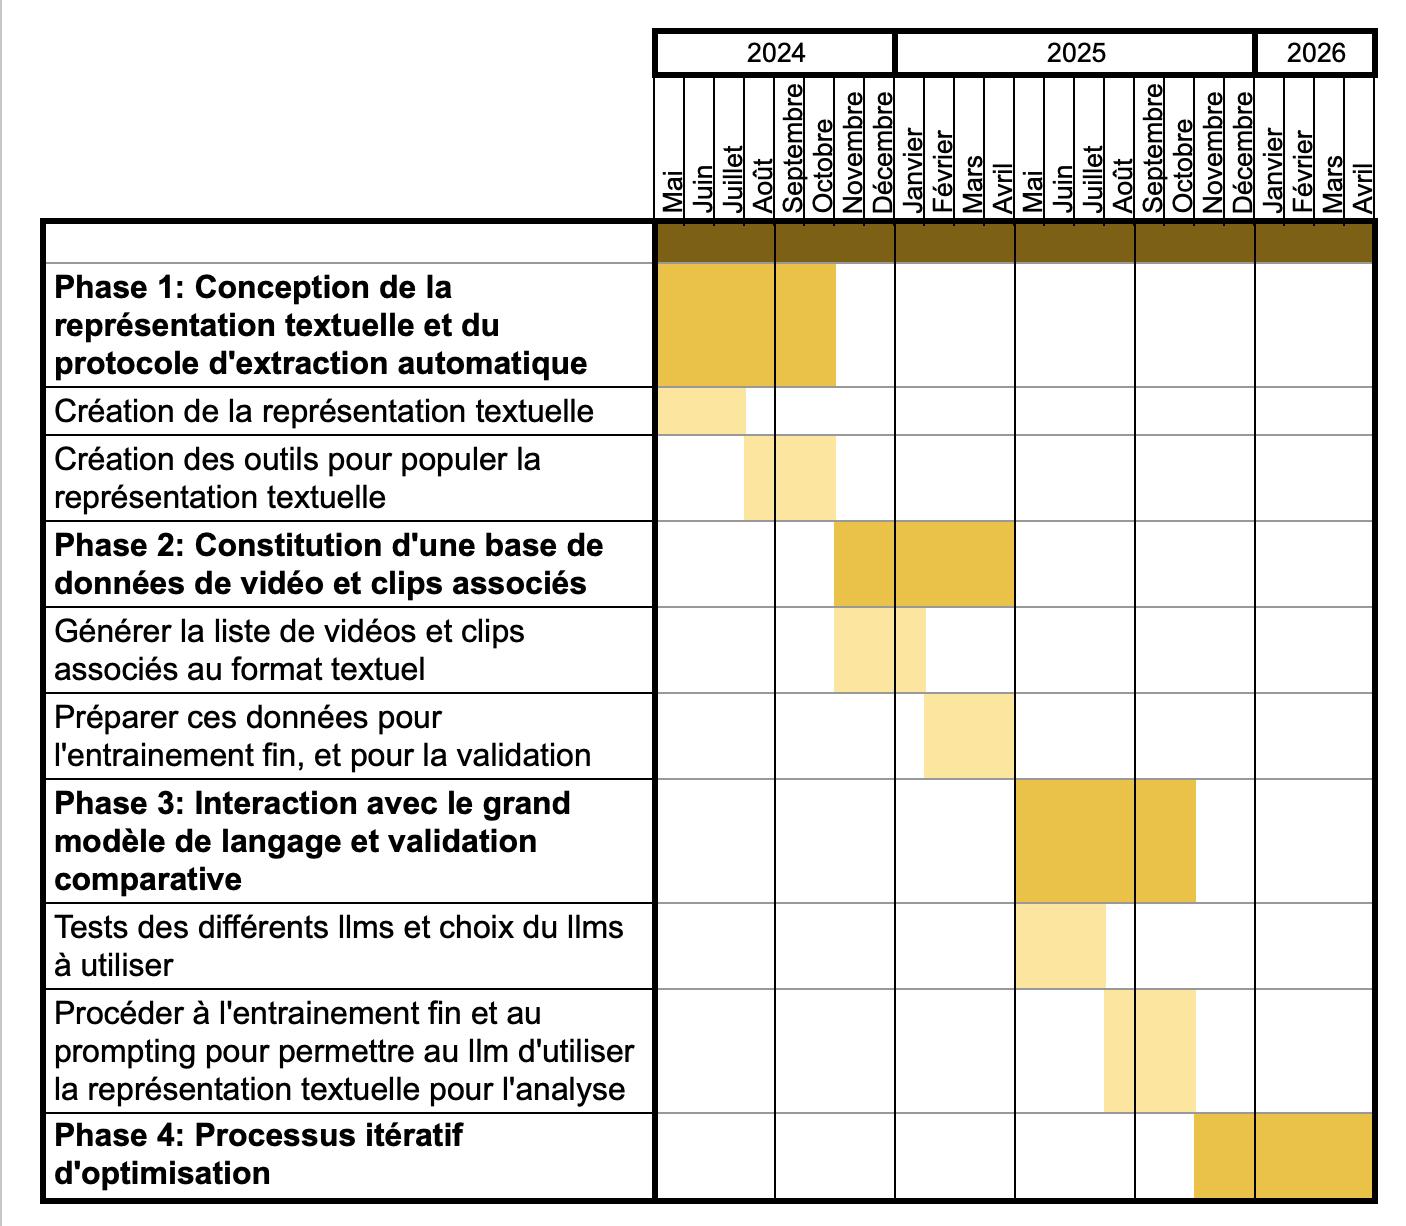
\includegraphics[width=1\textwidth]{source/gantt-v-fg.png}
  \caption{Échéancier du projet}
  \label{fig:label}
\end{figure}


